


\section{Auswertung}
\label{sec:auswertung}

In diesem Kapitel werden die aufgenommenen Messwerte ausgewertet.





\subsection{Resonatorstabilität}
\label{sec:resonatorstabilität}


In diesem Abschnitt wird die Stabilitätsbedinung hinsichtlich der maximal möglichen Resonatorlänge überprüft.
Die maximalen Resonatorlängen $L$, bei der der Laserbetrieb stabil war, finden sich in \autoref{tab:maximale Resonatorlängen}. 
Die verwendeten Spiegel hatten die Krümmungsradien $r_1$ und $r_2$.

\begin{table}
\centering
\caption{Maximale stabile Resonatorlängen L für Spiegel mit Krümmungsradius $r_1$ und $r_2$}
\begin{tabular}{c c c}
\toprule
{$L$[cm]} & {$r_1$[mm]} & {$r_2$[mm]}\\
\midrule
204,0  &  1400 & 1400\\
139,5  &  $\infty$ & 1400\\
\bottomrule
\label{tab:maximale Resonatorlängen}
\end{tabular}
\end{table}



Aus der Stabilitätsbedingung aus \autoref{sec:Resonator} ergeben sich die maximalen theoretisch stabilen Resonatorlängen zu:

\begin{equation}
L_{max} = \text{2,8}\,\text{m} \ \ \ \text{für}\  r_1, r_2 = 1400\,\text{mm}
\label{eq:Lmax1}
\end{equation}
\begin{equation}
L_{max} = \text{1,4}\,\text{m} \ \ \ \text{für}\  r_1 = \infty, r_2 = 1400\,\text{mm}
\label{eq:Lmax2}
\end{equation}









\subsection{TEM-Moden}
\label{sec:TEM-Moden}

Dieser Abschnitt behandelt die Auswertung der Messung zweier TEM-Moden.
Die Stromstärke der Photodiode ist proportional zur Lichtintensität und wird daher hier als Maß für selbige behandelt. Die Messung der Intensität für die Fundamentalmode $\text{TEM}_{00}$ finden sich in \autoref{tab:TEM_00}. Die der ersten Mode $\text{TEM}_{10}$, in die hier als $x$-Achse definierte Richtung, findet sich in \autoref{tab:TEM_10}.

\begin{table}
\centering
\caption{Messung der Intensitätsverteilung in Einheiten der Stromstärke zur $\text{TEM}_{00}$}
\begin{tabular}{c c}
\toprule
{$\Delta x$[mm]} & {$I$[$\mu$A]}\\
\midrule
-12	&	0,3	\\
-11	&	0,4	\\
-10	&	0,8	\\
-9	&	1,2	\\
-8	&	1,9	\\
-7	&	2,6	\\
-6	&	3,4	\\
-5	&	4,2	\\
-4	&	5,2	\\
-3	&	6,3	\\
-2	&	7,0	\\
-1	&	7,2	\\
0	&	7,2	\\
1	&	8,0	\\
2	&	7,4	\\
3	&	7,0	\\
4	&	6,4	\\
5	&	5,5	\\
6	&	4,4	\\
7	&	3,5	\\
8	&	2,6	\\
9	&	1,8	\\
10	&	1,3	\\
11	&	0,8	\\
12	&	0,5	\\
13	&	0,3	\\
\bottomrule
\label{tab:TEM_00}
\end{tabular}
\end{table}

\begin{table}
\centering
\caption{Messung der Intensitätsverteilung in Einheiten der Stromstärke zur $\text{TEM}_{10}$}
\begin{tabular}{c c}
\toprule
{$\Delta x$[mm]} & {$I$[$\mu$A]}\\
\midrule
-18	&	0,2	\\
-17	&	0,3	\\
-16	&	0,4	\\
-15	&	0,6	\\
-14	&	0,8	\\
-13	&	1,0	\\
-12	&	1,2	\\
-11	&	1,5	\\
-10	&	1,6	\\
-9	&	1,7	\\
-8	&	1,6	\\
-7	&	1,2	\\
-6	&	1,1	\\
-5	&	0,8	\\
-4	&	0,5	\\
-3	&	0,2	\\
-2	&	0,1	\\
-1	&	0,0	\\
0	&	0,1	\\
1	&	0,3	\\
2	&	0,5	\\
3	&	0,9	\\
4	&	1,2	\\
5	&	1,5	\\
6	&	1,8	\\
7	&	2,0	\\
8	&	2,0	\\
9	&	1,9	\\
10	&	1,8	\\
11	&	1,5	\\
12	&	1,3	\\
13	&	1,0	\\
14	&	0,8	\\
15	&	0,6	\\
16	&	0,5	\\
17	&	0,4	\\
18	&	0,2	\\
\bottomrule
\label{tab:TEM_10}
\end{tabular}
\end{table}


\clearpage

Die Funktion $I_{00}$ wurde an die Messwerte aus \autoref{tab:TEM_00} angepasst, die Funktion $I_{10}$ an die aus \autoref{tab:TEM_10}, um den theoretischen Verlauf mit den Messwerten verlgeichen zu können.

\begin{equation}
I_{00}(x) = A \cdot e^{-(\frac{x-x_0}{w})^{2}}
\label{eq:I_00}
\end{equation}

\begin{equation}
I_{10}(x) = 2A \cdot (\frac{x-x_0}{w})^{2} \cdot e^{-(\frac{x-x_0}{w})^{2}}
\label{eq:I_10}
\end{equation}

Die Parameter für \autoref{eq:I_00} ergaben sich zu:
\begin{equation}
A = 7,88 \pm 0,05 \,\mu \text{A}
\end{equation}
\begin{equation}
x_0 =  0,57 \pm 0,04\, \text{mm}
\end{equation}
\begin{equation}
w = 7,09 \pm 0,05\, \text{mm}
\end{equation}



Für \autoref{eq:I_10} berechneten sich die Parameter zu:
\begin{equation}
A = 2,43 \pm 0,06 \,\mu \text{A}
\end{equation}
\begin{equation}
x_0 =  -0.67 \pm 0,12\, \text{mm}
\end{equation}
\begin{equation}
w = 8.35 \pm 0,12\, \text{mm}
\end{equation}




In \autoref{fig:TEM_00} sind der Fit der Funktion $I_{00}$ und die Messwerte zur Fundamentalmode aus \autoref{tab:TEM_00} aufgetragen. Die Messwerte aus \autoref{tab:TEM_10} und der Fit der Funktion $I_{10}$ sind in \autoref{fig:TEM_10} zu sehen.


\begin{figure}
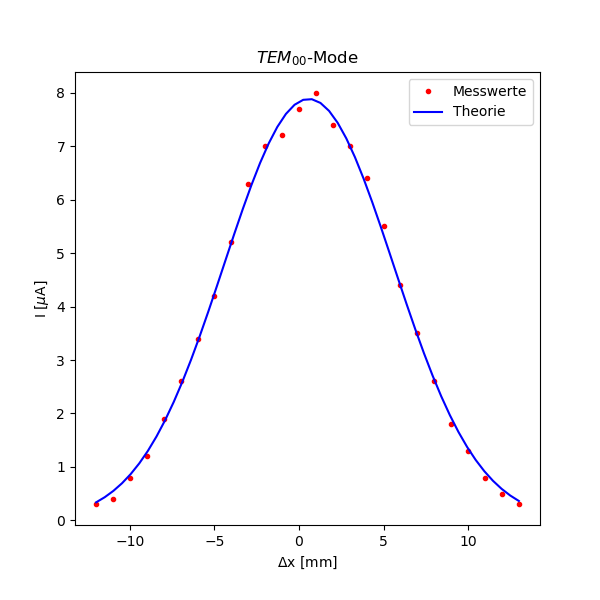
\includegraphics{figures/TEM_00.png}
\caption{Messung und theoretische Werte der $\text{TEM}_{00}$}
\label{fig:TEM_00}
\end{figure}


\begin{figure}
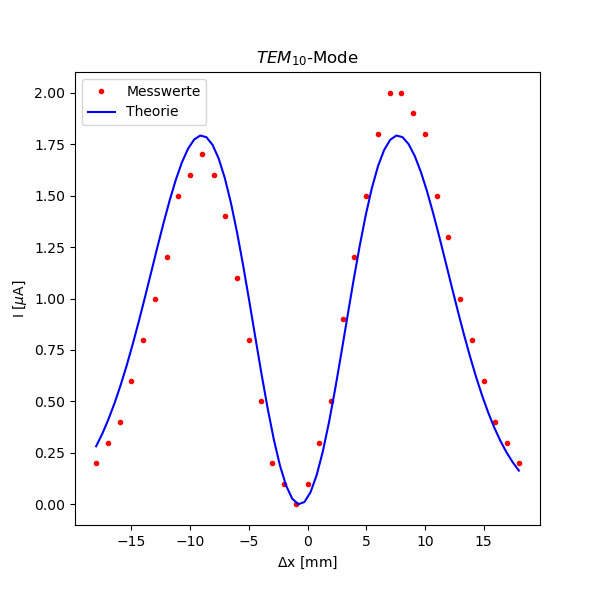
\includegraphics{figures/TEM_10.png}
\caption{Messung und theoretische Werte der $\text{TEM}_{10}$}
\label{fig:TEM_10}
\end{figure}










\clearpage
 
\subsection{Polarisation}
\label{sec:Polarisation}

Dieser Abschnitt befasst sich mit der Auswertung der Polarisation des Lasers. Die gemessene Stahlungsleistung $P$ zu verschiedenen Polarisationswinkeln $\phi$ ist in \autoref{tab:Polarisation} zu sehen. Der Startwinkel $\phi = 0$\,° wurde dabei willkürlich zu Beginn der Messung festgelegt.


\begin{table}
\centering
\caption{gemessene Strahlungsleistung $P$ zu verschiedenen Polarisationswinkeln $\phi$}
\begin{tabular}{c c c c}
\toprule
{$\phi$[°]} & {$P$[mW]} & {$\phi$[°]} & {$P$[mW]}\\
\midrule
0	&	0,0	&	92	&	3,9	\\
4	&	0,1	&	96	&	3,7	\\
8	&	0,2	&	100	&	3,5	\\
12	&	0,3	&	104	&	3,4	\\
16	&	0,4	&	108	&	3,3	\\
20	&	0,6	&	112	&	3,1	\\
24	&	0,8	&	116	&	2,9	\\
28	&	1,0	&	120	&	2,7	\\
32	&	1,2	&	124	&	2,4	\\
36	&	1,5	&	128	&	2,2	\\
40	&	1,8	&	132	&	1,9	\\
44	&	2,0	&	136	&	1,6	\\
48	&	2,3	&	140	&	1,4	\\
52	&	2,6	&	144	&	1,1	\\
56	&	2,8	&	148	&	0,9	\\
60	&	3,0	&	152	&	0,8	\\
64	&	3,3	&	156	&	0,5	\\
68	&	3,5	&	160	&	0,4	\\
72	&	3,6	&	164	&	0,2	\\
76	&	3,7	&	168	&	0,1	\\
80	&	3,8	&	172	&	0,1	\\
84	&	3,9	&	176	&	0,0	\\
88	&	3,9	&	180	&	0,1	\\
\bottomrule
\label{tab:Polarisation}
\end{tabular}
\end{table}


Die Funktion \autoref{eq:Polarisationsfit} wurde an die gemessenen Werte aus \autoref{tab:Polarisation} angepasst und beides danach in \autoref{fig:Polarisation} dargestellt.


\begin{equation}
P(\phi) = P_0\cdot(\cos(\phi - \phi_0)^{2}
\label{eq:Polarisationsfit}
\end{equation}

Es ergaben sich die Parameter wie folgt:
\begin{equation}
P_0 = (\text{3,83} \pm \text{0,01})\,\text{mW}
\end{equation}
\begin{equation}
\phi_0 = (\text{86,82} \pm \text{0,15})\,\text{°}
\end{equation}


\begin{figure}
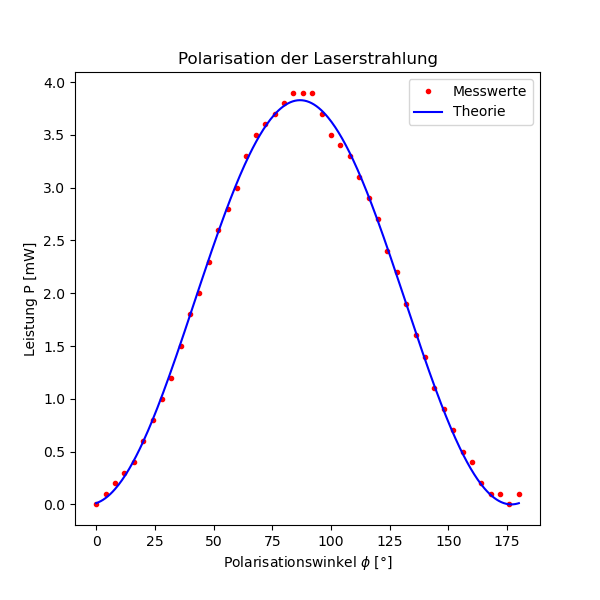
\includegraphics{figures/Polarisation.png}
\caption{Messung und theoretische Werte der Polarisation des Laserstrahls}
\label{fig:Polarisation}
\end{figure}







\clearpage

\subsection{Multimodenbetrieb}
\label{sec:Multimodenbetrieb}

In diesem Abschnitt werden die Schwebungsfrequenzen, der longitudinalen Moden ausgewertet. 
Die durch den Spektrumanalysator zu verschiedenen Resonatorlängen $L$ gemessenen Schwebungsfrequenzen finden sich in \autoref{tab:Multimoden}.


\begin{table}
\centering
\caption{Schwebungsfrequenzen $\nu_i$ zu verschiedenen Resonatorlängen $L$}
\begin{tabular}{c c c c c c c}
\toprule
$L$ [cm]	&	202,6	&	190,7	&	182,0	&	167,6	&	158,2	&	140,4	\\
\midrule
$\nu_1$[MHz]	&	225	&	233	&	244	&	90	&	94	&	105	\\
$\nu_2$[MHz]	&	443	&	469	&	495	&	180	&	188	&	214	\\
$\nu_3$[MHz]	&	664	&	701	&	730	&	270	&	285	&	319	\\
$\nu_4$[MHz]	&	881	&	938	&	979	&	353	&	375	&	424	\\
$\nu_5$[MHz]	&		&		&		&	446	&	473	&	529	\\
$\nu_6$[MHz]	&		&		&		&	533	&	566	&	634	\\
$\nu_7$[MHz]	&		&		&		&	623	&	660	&	739	\\
$\nu_8$[MHz]	&		&		&		&	713	&	750	&	844	\\
$\nu_9$[MHz]	&		&		&		&	799	&	844	&	953	\\
$\nu_{10}$[MHz]	&		&		&		&	885	&	941	&	1058	\\
$\nu_{11}$[MHz]	&		&		&		&	979	&	1035	&	1163	\\
&		&		&		&		&		&\\
											\midrule		
&		&		&		&		&		&\\		
$L$ [cm]	&	116,9	&	107,4	&	96,2	&	80,2	&	61,8	&	40,5	\\
\midrule
$\nu_1$[MHz]	&	128	&	139	&	154	&	184	&	236	&	90	\\
$\nu_2$[MHz]	&	255	&	278	&	311	&	368	&	473	&	270	\\
$\nu_3$[MHz]	&	383	&	416	&	461	&	551	&	709	&	360	\\
$\nu_4$[MHz]	&	506	&	551	&	615	&	735	&	945	&	446	\\
$\nu_5$[MHz]	&	634	&	690	&	769	&	919	&		&	630	\\
$\nu_6$[MHz]	&	761	&	829	&	923	&	1103	&		&	716	\\
$\nu_7$[MHz]	&	889	&	968	&	1076	&		&		&	799	\\
$\nu_8$[MHz]	&	1013	&	1103	&	1230	&		&		&		\\
$\nu_9$[MHz]	&		&		&		&		&		&		\\
$\nu_{10}$[MHz]	&		&		&		&		&		&		\\
$\nu_{11}$[MHz]	&		&		&		&		&		&		\\

\bottomrule
\label{tab:Multimoden}
\end{tabular}
\end{table}


Mittels linearer Regression lässt sich zu jeder Resonatorlänge die Grundfrequenz der Schwebungsfrequenzen ermitteln. Dafür wurde die Funktion \autoref{eq:linMultimoden} an die Messwerte aus \autoref{tab:Multimoden} angepasst. 

\begin{equation}
\nu (x) = m \cdot x + n
\label{eq:linMultimoden}
\end{equation}

Wobei $x$ das ganzzahlige Vielfache der Grundfequenz und $\nu (x)$ die gemessenen Schwebungsfrequenzen angibt. Graphisch beispielhaft für die Resonatorlänge $L = 167,6\,\text{cm}$ in \autoref{fig:linMultimoden} dargestellt.

\begin{figure}
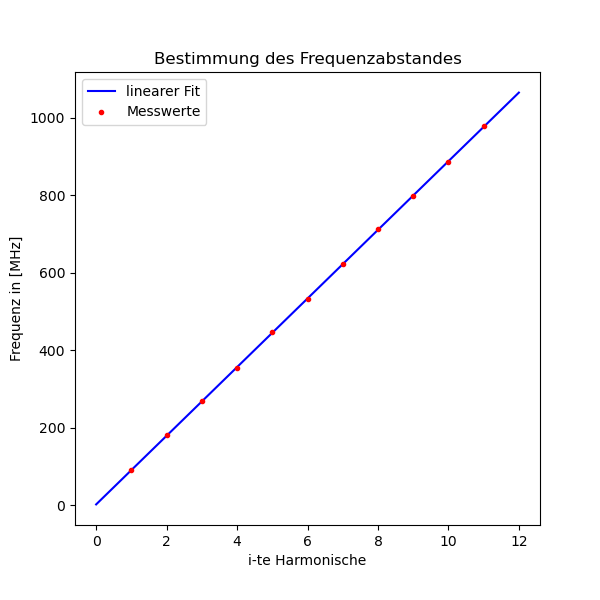
\includegraphics{figures/Frequenzabstand.png}
\caption{Gemessene Schwebungsfrequenzen und linearer Fit zur Resonatorlänge $L = 167,6\,\text{cm}$}
\label{fig:linMultimoden}
\end{figure}

Der Parameter $m$ entspricht dem Abstand zweier Schwebungsfrequenzen und damit der Grundfrequenz. Die Ergebnisse der Parameterbestimmung zur jeweiligen Resonatorlänge $L$ sind in \autoref{tab:linMultimoden} zu finden.



\begin{table}
\centering
\caption{Parameter der linearen Regression}
\begin{tabular}{c c}
\toprule

{$m$[MHz]}&{$n$[MHz]}\\
\midrule
{ 218,899 \pm 0,232 }& { 6,000 \pm 0,636 }\\
{ 234,699 \pm 0,293 }& { -1,499 \pm 0,803 }\\
{ 243,999 \pm 0,959 }& { 2,000 \pm 2,627 }\\
{ 88,627 \pm 0,188 }& { 1,963 \pm 1,275}\\
{ 93,918 \pm 0,170 }& { 1,127 \pm 1,153}\\
{ 105,618 \pm 0,121 }& { 1,018 \pm 0,822 }\\
{ 126,511 \pm 0,153 }& { 1,821 \pm 0,774 }\\
{ 137,809 \pm 0,154 }& { 1,607 \pm 0,778 }\\
{ 153,535 \pm 0,145 }& { 1,464 \pm 0,732 }\\
{ 183,771 \pm 0,049 }& { 0,133 \pm 0,191 }\\
{ 236,300 \pm 0,035 }& { 0,000 \pm 0,098 }\\
{ 117,464 \pm 4,238 }& { 3,143 \pm 18,955 }\\

\bottomrule
\label{tab:linMultimoden}
\end{tabular}
\end{table}


Der Frequenzabstand zweier longitudinaler Moden ist gegeben durch:

\begin{equation}
\delta \nu (L) = \frac{c}{2L}
\end{equation}

Wobei $c$ die Lichtgeschwindigeit ist. Diese Formel umgestellt nach $L$ erlaubt einen Fit der Funktion

\begin{equation}
L (\delta \nu) = \frac{c_0}{2\cdot \delta \nu}
\label{eq:fitMultimoden}
\end{equation}

mit $c_0$ als freiem Parameter und $m$ aus \autoref{tab:linMultimoden} als Werte für $\delta \nu$. Dabei wurden auch die Standardabweichungen für $m$ berücksichtigt. Die ersten drei Werte, sowie der letzte Wert für $m$ aus \autoref{tab:linMultimoden} weichen sichtlich stark von der Theorie ab und wurden daher zur Parameterbestimmung nicht miteinbezogen. Der Parameter $c_0$ ergab sich zu:

\begin{equation}
c_0 = (\text{299400884,188} \pm \text{9,146})\, \frac{\text{m}}{\text{s}}
\end{equation}

In \autoref{fig:Multimoden} sind der Fit der Funktion \autoref{eq:fitMultimoden} und die ermittelten Werte der Grundfrequenzen aus \autoref{tab:linMultimoden} zu sehen. Der Frequenzabstand $\delta \nu$ wurde hier mit $f$ bezeichnet.


\begin{figure}
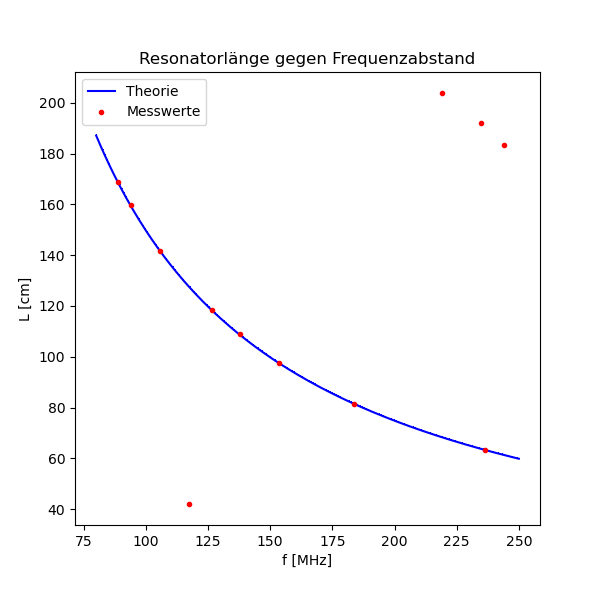
\includegraphics{figures/Multimoden.png}
\caption{Resonatorlänge $L$ und Abstand zweier longitudinaler Moden $f$: Messwerte und theoretische Werte}
\label{fig:Multimoden}
\end{figure}







\clearpage

\subsection{Wellenlänge}
\label{sec:Wellenlänge}

In diesem Abschnitt wird die Messung der Abstände der Beugungsmaxima ausgewertet, um daraus die Wellenlänge der Laserstrahlung zu bestimmen.
Die Messung für ein Gitter mit $100$\,lines/mm und eines mit $600$\,lines/mm ist in \autoref{tab:WellenAbstand} zu sehen.

\begin{table}
\centering
\caption{Abstände der Beugungsmaxima für zwei verschiedene Gitter}
\begin{tabular}{c c}
\toprule
$100\,$lines/mm&$600\,$lines/mm\\
$\delta x$[cm]&$\delta x$[cm]\\
\midrule
2,1	&	22,9	\\
2,1	&	22,9	\\
2,1	&		\\
2,1	&		\\
2,1	&		\\
2,1	&		\\
\bottomrule
\label{tab:WellenAbstand}
\end{tabular}
\end{table}

Innerhalb der Messgenauigkeit gab es keinen Unterschied zwischen den gemessenen Abständen für ein Gitter. Daher ergeben sich die Mittelwerte direkt zu:

\begin{equation}
x_1 = \text{2,1}\,\text{cm}
\end{equation}
\begin{equation}
x_2 = \text{22,9}\,\text{cm}
\end{equation}


Der Abstand zwischen Gitter und Schirm für die erste Messreihe betrug $l = 31,6$\,cm und $l = 55,7$\,cm für die zweite. Zur Berechnung der Wellenlänge wird die folgende Formel\footnote{https://www.leifiphysik.de/optik/beugung-und-interferenz/grundwissen/vielfachspalt-und-gitter} verwendet

\begin{equation}
\lambda = \frac{d\cdot \delta x}{\sqrt{l^{2} +  (\delta x)^{2}}}
\end{equation}

 wobei $d$ den Abstand zwischen zwei Spalten des Gitters bezeichnet. Dieser lässt sich jeweils aus dem Kehrwert von $100$\,lines/mm bzw $600$\,lines/mm berechnen. Daraus ergeben sich die Wellenlängen der beiden Messungen zu:

\begin{equation}
\lambda = \text{663,1}\,\text{nm}
\end{equation}
\begin{equation}
\lambda = \text{633,7}\,\text{nm}
\end{equation}


\clearpage




































